\hfill\break
\justifying
Siguiendo en el orden de secciones, se encuentran las operaciones capaces de adicionar ruido a las imagenes.´

\hfill\break
\justifying
Aún cuando el ruido en una imagen es un factor detrimental, es una situación muy común en la captura de imagenes por lo que su estudio es también importante y es así que se agregan la funcionalidad para adicionamiento de ruido.

\hfill\break
\justifying
El ruido, como cualquier entidad o resultado que es intermedio en una imagen capturada, no es de interes para los propósitos del cómputo principal, por lo que se suele definir al ruido como toda a quella situación que entorpece en cualquiera de las etapas, al tratamiento de las imágenes.

\hfill\break
\justifying
Con diversas causantes que pueden generar ruido en nuestras imagenes, se mencionan los tipos de ruidos clasificados en 3:
\begin{itemize}
	\item \textbf{Aditivo}: Se adiciona al azar a cada pixel de la imagen $f(x,y)$, un valor real \textit{c}, de forma que: $\overbrace{f}(x,y) = f(x,y)+c$.
	
	\textbf{Substractivo}: Se resta en este caso, al azar a cada pixel de la imagen $f(x,y)$, un valor real \textit{c}, de forma que: $\overbrace{f}(x,y) = f(x,y)-c$
	
	\textbf{Mezclado}: Se adiciona o resta al azar a cada pixel de la imagen $f(x,y)$, un valor real \textit{c}, de forma que: $\overbrace{f}(x,y) = f(x,y)+c$ o $\overbrace{f}(x,y) = f(x,y)-c$
\end{itemize}

\hfill\break
\justifying
Con la finalidad de estudiarlos y entender las técnicas que pueden ayudar a contrarrestrarlos, se añaden los ruidos más comunes:

\subsection*{Ruido Gausiano}
	\hfill\break
	\justifying
	Produce pequeñas variaciones en la image, generalmente tiene origen en los componentes electrónicos. Afecta a la imagen completa donde la desnsidad de todos los pixeles se ve alterada. Cada muestra de entrada es afectada por un valor diferente, desde cero hasta un valor de saturación mínimo o máximo.
	
	\hfill\break
	\justifying
	Este tipo de ruido mezclado, sigue un comportamiento gausiano, de forma que la variable \textit{c} toma valores según la siguiente relación:
	\begin{equation*}
		c = (L-1)exp\left( \frac{-z^2}{2\sigma^2} \right)
	\end{equation*}

\subsection*{Ruido Sal y Pimienta}
	\hfill\break
	\justifying
	El valor que toma el pixel no tiene relación con el valor real, sino que toma valores muy altos o muy bajos. Tomando el máximo(sal) o el mínimo(pimienta). Se produce normalmente en la cuantificación que se realiza en el proceso de digitalización.
	
	\hfill\break
	\justifying
	Como este tipo de ruido se caracteriza por saturar el valor de uno o más pixeles de la imagen hacia los límites positivos o límite inferior, su asignación se realiza en el programa de forma aleatoria con el valor de \textit{l} como limitante de cuanto ruido de este tipo adicionar

\subsection*{Implementacion ruido}
\hfill\break
\justifying
La implementación del proceso de adicionado de ruido para cada tipo es diferente, más sin embargo se conjuntan ambos en 1 sola función por la facilidad que ofrece este tipo de implementación. Para adicionar uno u otro, se pasa un parámetro tipo \textit{string} con la cadena \textit{'gaussian'} o \textit{'s\&p'} para escoger el tipo, mientras que los parámetros de cada uno se pasa como valor con llave, situación en la que Python deja su adición en la llamada a la función sin poner límite a estos mientras se especifique la lista en la definición de la función.

\newpage

	\begin{landscape}
		\begin{figure}[!h]
			\begin{tabular}{cc}
				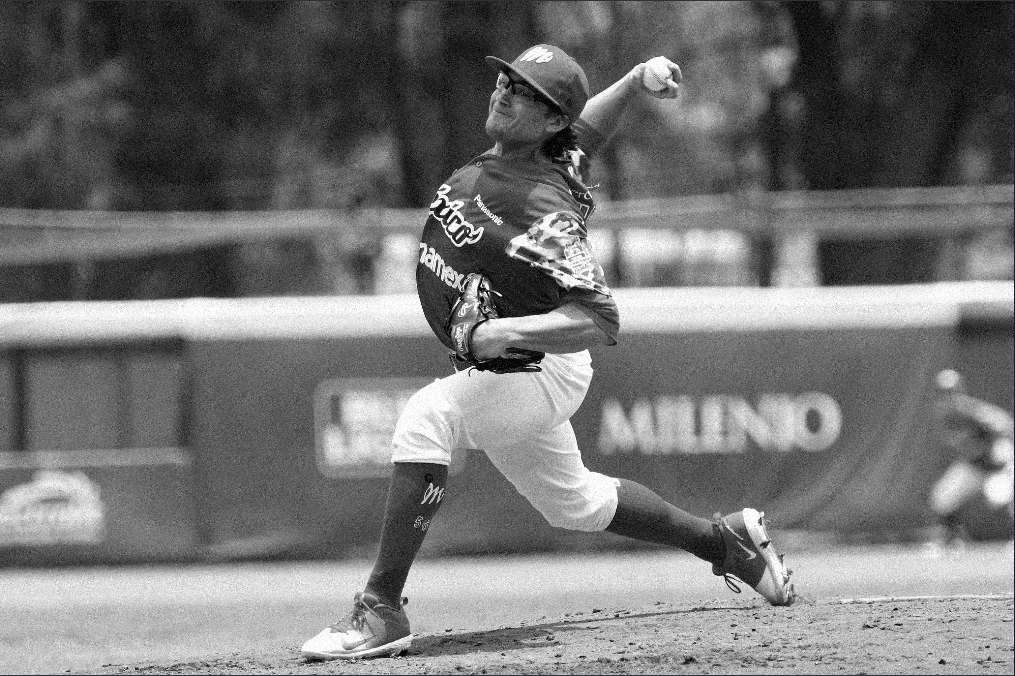
\includegraphics[width=12.25cm]{Imagenes/Ruido_gauss_bn_1.png} & 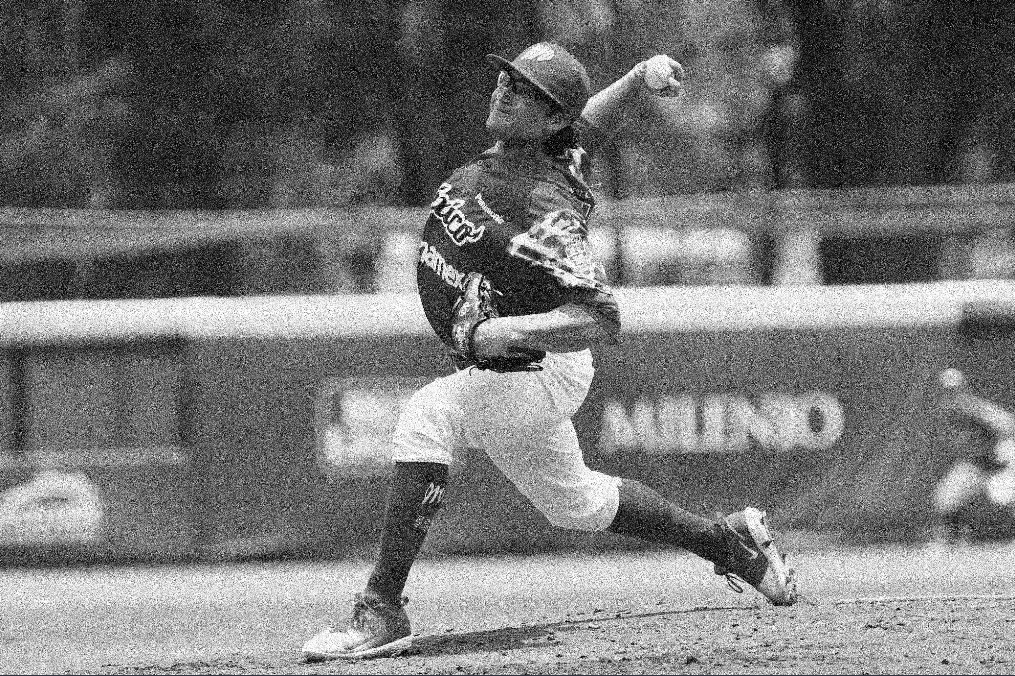
\includegraphics[width=12.25cm]{Imagenes/Ruido_gauss_bn_2.png} \\
				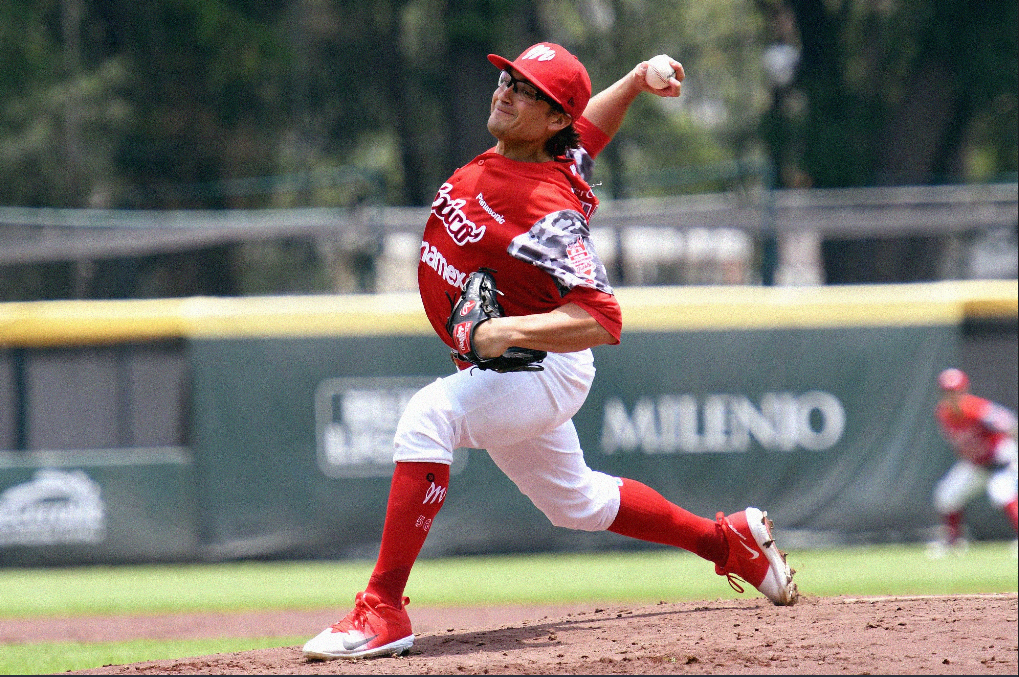
\includegraphics[width=12.25cm]{Imagenes/Ruido_gauss_color_1.png} & 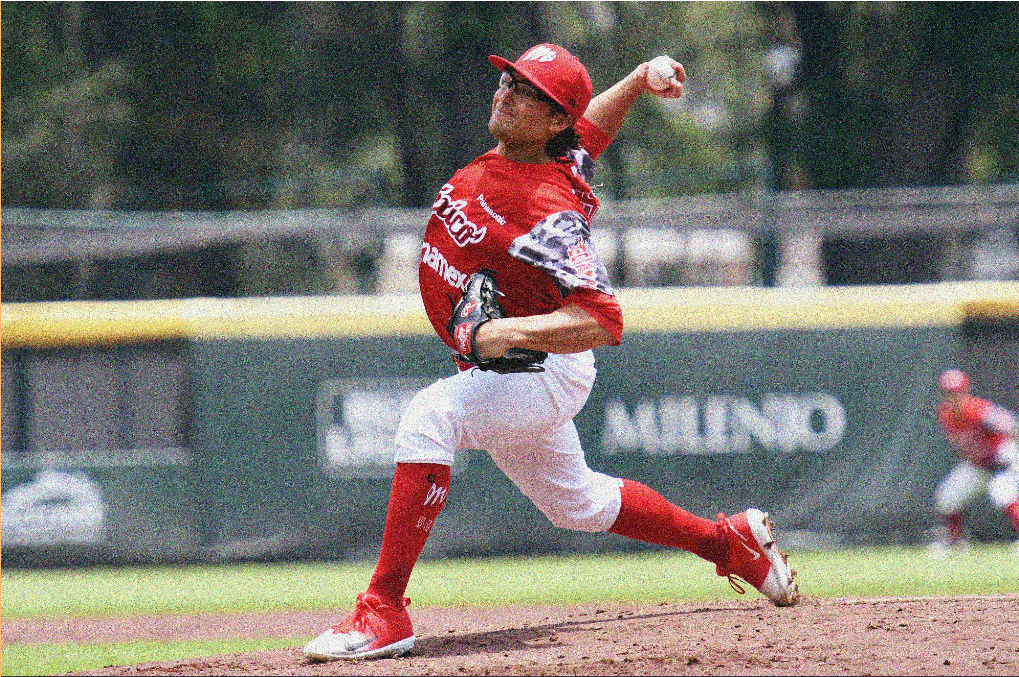
\includegraphics[width=12.25cm]{Imagenes/Ruido_gauss_color_2.png}
			\end{tabular}
			\label{Ruido_Gauss}
			\caption{Ejemplo de imágenes a escala de grises y a color, con ruido tipo gaussiano adicionado \\ 1) Imagen en escala de grises con parámetros $\mu= 3$ y $\sigma = 15$ \\ 2) Imagen en escala de grises con parámetros $\mu= 5$ y $\sigma = 50$ \\ 3) Imagen a color con parámetros $\mu = 3$ y $\sigma = 15$ \\ 4)Imagen a color con parámetros $\mu = 5$ y $\sigma = 50$}
		\end{figure}
	\end{landscape}

	\begin{landscape}
		\begin{figure}[!h]
			\begin{tabular}{cc}
				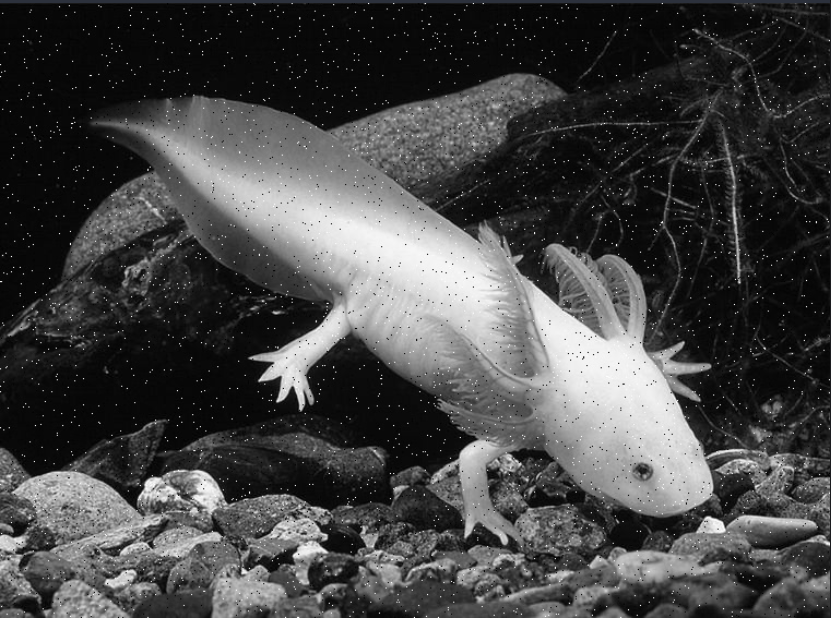
\includegraphics[width=11cm]{Imagenes/Ruido_sp_bn_1.png} & 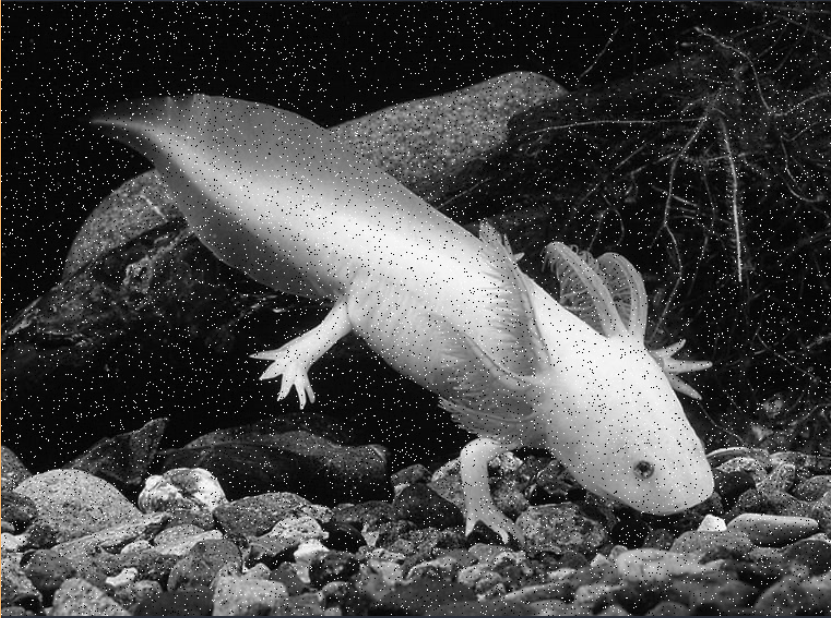
\includegraphics[width=11cm]{Imagenes/Ruido_sp_bn_2.png} \\
				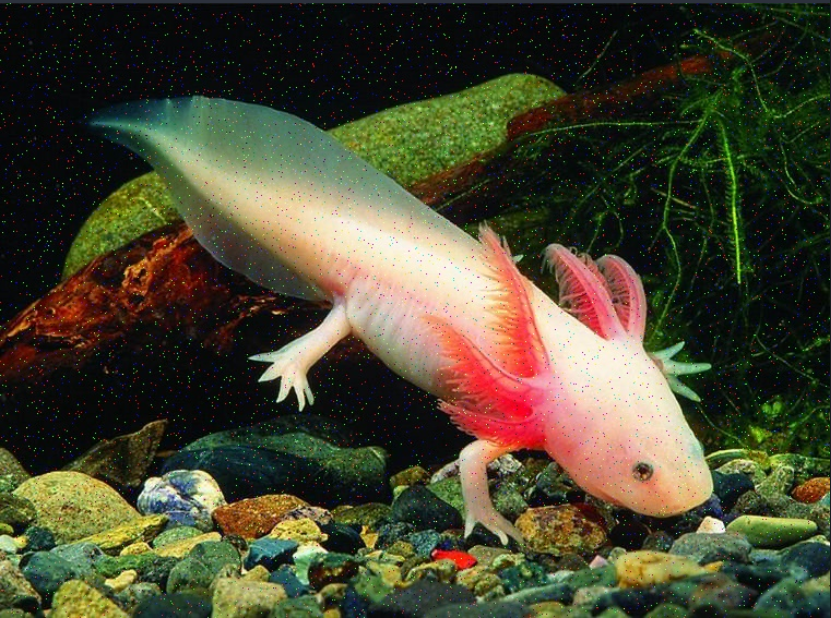
\includegraphics[width=11cm]{Imagenes/Ruido_sp_color_1.png} & 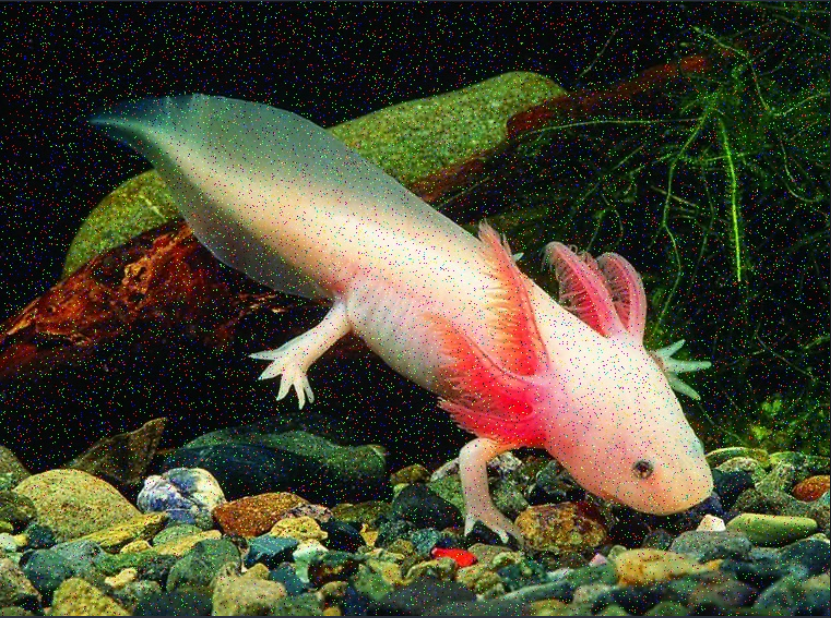
\includegraphics[width=11cm]{Imagenes/Ruido_sp_color_2.png}
			\end{tabular}
			\label{Ruido_sal_pimienta}
			\caption{Ejemplo de imágenes a escala de grises y a color, con ruido tipo sal y pimienta adicionado \\ 1) Imagen en escala de grises con parámetro $l = 150$ \\ 2) Imagen en escala de grises con parámetro $l = 50$ \\ 3) Imagen a color con parámetro $l = 150$ \\ 4)Imagen a color con parámetro $l = 50$}
		\end{figure}
	\end{landscape}
	
	\begin{lstlisting}[language=Python]
		def noise(noise_type:str,image,**kargs):
			list_keys = list(kargs)
			image = copy(image)
			
			if noise_type == "gaussian":
				# Obtains the values of the mean and standard deviation
				mean = kargs['mean'] if 'mean' in list_keys else 0; std_deviation = kargs['std_deviation'] if 'std_deviation' in kargs.keys() else 0.1
				print('mean >>',mean,'  std deviation >>',std_deviation)
				# Creates the noise in a random manner according to the normal distribution with the given mean and standard deviation
				gauss = random.normal(mean,std_deviation,image.shape)
				# The noise gets added
				noisy_image = image + gauss
				# Rectifies that values an the upper and lower limit do not exceeds 0-255
				noisy_image[noisy_image > 255] = 255; noisy_image[noisy_image < 0] = 0
				return noisy_image.astype(uint8)
			elif noise_type == "s&p":
				l = 101 if 'l' not in list_keys else kargs['l']
				# Convert the image to 0 to 1 float to avoid wrapping that occurs with uint8
				image.astype(float16, copy = False)
				image = multiply(image, (1/255))
				# Generate noise to be added to the image
				noise = random.randint(l, size=image.shape)
				# Convert high and low bounds of l in noise to salt and pepper noise then add it to
				# our image. 1 is subtracted from l to match bounds behaviour of random.randint.
				image = where(noise == 0, 0, image)
				image = where(noise == (l-1), 1, image)
				# Properly handles the conversion from float16 back to uint8
				image = cv2.convertScaleAbs(image, alpha = (255/1))        
				return image
	\end{lstlisting}
	
	\hfill\break
	\justifying
	La implementación del ruido gausiano es bastante sencilla y muy conveniente si se apoya de la herramienta que provee la biblioteca numpy en su módulo random. La función \textit{normal}, genera un array con valores tomados de forma aleatoria de una distribución normal con una cierta media y desviación estándar dada para una cierta dimensionalidad.
	
	\hfill\break
	\justifying
	Lo que resta una vez creados estos valores, es realizar la suma elemento por elemento con la imagen, y con esta acción se ha adicionado el ruido con distribución gausiana. Importante la penúltima instrucción que va a rectificar aquellos valores en la nueva imagen con ruido, que excedan los límites superiores(255) e inferior(0).
	
	\hfill\break
	\justifying
	Finalmente la adición del ruido sal y pimienta inicia convirtiendo el arreglo de la imagen en valores enteros a un tipo de dato float y se realiza la normalización, esto para evitar errores en la asignación de los nuevos valores.
	
	\hfill\break
	\justifying
	Al igual que sucede con el ruido gausiano, el trabajo se auxilia de la herramienta aleatoria disponible en numpy que permite generar un arreglo de tamaño igual al número de elementos en la imagen, definiendo el número más alto que puede tomarse y simplemente se asigna al pixel el valor 0 cuando en el mismo índice el arreglo del ruido tiene el valor 0. De forma similar, cuando el indice del arreglo de ruido tiene el valor del límite especificado menos 1, la imagen toma el valor saturado en ese pixel.
	
	\hfill\break
	\justifying
	Resta únicamente escalar de vuelta los valores del rango 0.0-1.0 a 0-255, y se retorna la imagen adicionada con ruido.